\documentclass[11pt]{article}
\usepackage[utf8]{inputenc}
\usepackage[T1]{fontenc}
\usepackage{fixltx2e}
\usepackage{graphicx}
\usepackage{longtable}
\usepackage{float}
\usepackage{wrapfig}
\usepackage{soul}
\usepackage{textcomp}
\usepackage{marvosym}
\usepackage{wasysym}
\usepackage{latexsym}
\usepackage{amssymb}
\usepackage{hyperref}
\tolerance=1000
\usepackage{fullpage}
\providecommand{\alert}[1]{\textbf{#1}}

\title{Report on the Relativity Experiments}
\author{Craig Roy}
\date{\today}
\hypersetup{
  pdfkeywords={},
  pdfsubject={},
  pdfcreator={Emacs Org-mode version 7.9.3f}}

\begin{document}

\maketitle


\section*{Experiment 1: Digital Clocks}
\label{sec-1}
\subsection*{Description}
\label{sec-1-1}

This simple time-dilation experiment consists of two `clocks' showing how the time experienced by a clock moving at a relativistic speed specified by the user in the `vField'.
\subsection*{How it works}
\label{sec-1-2}
\subsubsection*{Variables}
\label{sec-1-2-1}

\begin{itemize}
\item \emph{v} is the speed of the moving clock which is specified by the user.
\item \emph{t} is the time shown on the slower, moving clock. It is used to calculate t2.
\item \emph{t2} is the time shown on the static clock, it is calculated for each evolution, by multiplying \emph{t} by the lorentz factor, $\gamma$.
\end{itemize}
\subsubsection*{Evolution}
\label{sec-1-2-2}

The independant variable which is incremented at each evolution is \emph{t}. The animation runs at 20fps, incrementing \emph{t} by 0.05 each time, meaning that \emph{t} increases by 1 second per second.
The variable \emph{t2} increments at $\frac{0.05 \gamma}{frame}$, so $\gamma$ seconds per second.
\subsubsection*{UI}
\label{sec-1-2-3}

In the `control panel' on top, the UI consists of a field in which the user can enter the speed of the moving clock, along with pause and reset buttons.
In the bottom `time panel', the time passed for both the moving and the static clocks is shown. These time fields display the values to one decimal point as a number of seconds.
\begin{figure}[htb]
\centering
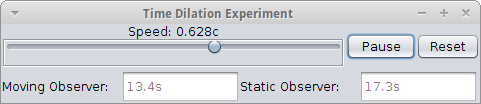
\includegraphics[width=.9\linewidth]{./DigitalUI.png}
\caption{UI of the digital clock experiment}
\end{figure}
\section*{Experiment 2: Analogue Clocks}
\label{sec-2}
\subsection*{Description}
\label{sec-2-1}

This experiment is very similar to the previous one, but the information is displayed with model analogue clocks rather than digital displays. Hopefully, this is a clearer demonstration of the concept at hand, and more fun to watch.
In this experiment the moving clock runs at 1 second per second, and the static clock runs faster, whereas in the previous experiment, the static clock ran at 1 second per second and the moving clock ran slower.
\subsection*{How it works}
\label{sec-2-2}
\subsubsection*{Variables}
\label{sec-2-2-1}

\begin{itemize}
\item \emph{v} is the speed of the moving clock which is entered by the user.
\item \emph{tic} is designed to be the independent variable in the ODE page. It is equivalent to the angle in degrees from the 12th hour on the slower moving clock.
\item \emph{a1} is the angle from the 12th hour of the slower moving clock in radians. It is calulated by $\frac{tic \times \pi}{180}$.
\item \emph{x1}, \emph{y1} are the x and y coordinates of the slower clock's hands. They are calculated from \emph{a1} using trigonometry in the fixed relations page.
\item \emph{lorentz} is the lorentz factor, $\gamma$, dependant on the speed entered by the user.
\item \emph{a2} is the angle from the 12th hour of the faster clock in radians. It is found by $\gamma$ \texttimes{} \emph{a1}.
\item \emph{x2}, \emph{y2} are the angles needed for the hands of the faster clock. Calculated using \emph{a2} rather than \emph{a1}.
\end{itemize}
\subsubsection*{Evolution}
\label{sec-2-2-2}

The variables \emph{a1} and \emph{a2} evolve according to the independant variable \emph{tic}. In \emph{a1}, simply converts \emph{tic} to radians and \emph{a2} multiplies \emph{a1} by $\gamma$.
The simulation runs at 6fps, where \emph{tic} is incremented by 1 every frame. This means that the angle of the hand on the slower clock increases by 6\textdegree{} every second. 6\textdegree{} is the angle between 1 second increments on an analogue clock.
From the increments in \emph{a1} and \emph{a2}, the corresponding \emph{x} and \emph{y} values are calculated using the fixed relations $x = -0.5\cos(a)$ and $y = 0.5\sin(a)$.
\subsubsection*{UI}
\label{sec-2-2-3}

The experiments UI consists of three windows:
\begin{itemize}
\item \emph{Spaceship Clock} shows time moving at 1 second per second in the moving rest frame.
\item \emph{Earth Clock} shows time in the static observer frame accelerated by a lorentz factor.
\item \emph{Control Panel} contains a field for the user to input the speed of the moving (spaceship) frame, a play/pause button and a reset button.
\end{itemize}
\begin{figure}[htb]
\centering
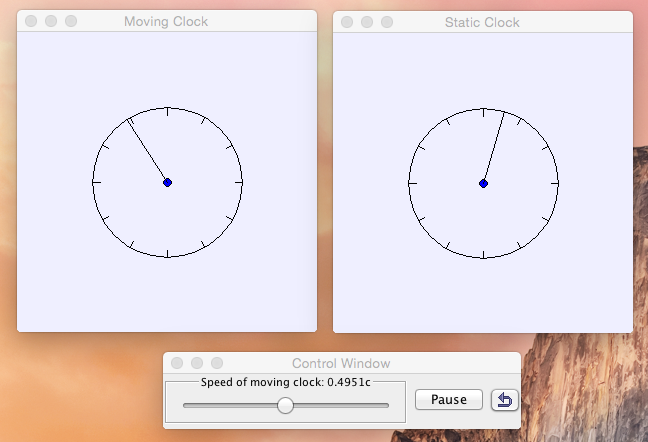
\includegraphics[width=.9\linewidth]{./analogueUI.png}
\caption{UI of the analogue clock simulation}
\end{figure}
\section*{Experiment 3: Photon Clock}
\label{sec-3}
\subsection*{Description}
\label{sec-3-1}

This experiment involves the concept of a photon clock. A photon clock is a device which measures the passage of time when a photon hits a sensor.

In this experiment there is a stationary clock (the lab clock) and a moving photon clock (the moving clock) 
   
\subsection*{How to use it}
\label{sec-3-2}

The slider can be used to adjust the speed of the clock in the moving frame. Observe how at speeds very close to the speed of light, the width of the moving photon clock changes.
The times measured by the two clocks are shown in a third window, and so is the Lorentz factor of the second clock and the speed.
\subsection*{How it works}
\label{sec-3-3}
\subsubsection*{Variables}
\label{sec-3-3-1}
\begin{itemize}

\item Simulation variables
\label{sec-3-3-1-1}%
\begin{itemize}
\item \emph{x, vx} are the position and velocity of the moving photon clock system along the x-axis within the frame. The \emph{x} position of the clock is incremented by $vx\dot dt$.
\item \emph{y, vy} are the position and velocity of the photon in the y-axis for the lab clock. \emph{y} is incremented by $vy\dot dt$ for each evolution of the system.
\item \emph{y2, vy2} are the position and velocity of the photon in the y-axis for the moving photon clock system. \emph{y2} is incremented by $vy2\dot dt2$ each evolution of the system.
\item \emph{lorentz} is the value of the Lorentz factor for the moving clock based on the speed of the clock as specified by the user
\item \emph{t} is the time observed by the lab clock.
\item \emph{dt} is the interval in which the lab clock is incremented.
\item \emph{t2} is the time observed by the moving clock.
\item \emph{dt2} is the interval with which the variables in the moving clock system are incremented. It is defined as $\frac{dt}{\gamma}$.
\end{itemize}


\item Length scaling variables
\label{sec-3-3-1-2}%
\begin{itemize}
\item \emph{mirror} is the width of the mirrors in the moving clock window. It is a fixed relation $\frac{2.5}{\gamma}$ so it varies with the speed of the system in order to demonstrate length contraction.
\item \emph{photon} is the width of the photon in the moving clock window. It is of the fixed relation $\frac{0.5}{\gamma}$ so that it also shrinks at high speeds in order to demonstrate length contraction.
\item \emph{upper} is point at which the photon should hit the upper mirror and start moving in the opposite direction.
\item \emph{lower} is the point at which the photon should hit the lower mirror and start moving in the opposite direction.
\end{itemize}
\end{itemize} % ends low level
\subsubsection*{Evolution}
\label{sec-3-3-2}

    Like the previous simulations, this simulation runs at 20fps. The evolution of this system is specified with code, rather than ODEs. There are two time variables \emph{t} and \emph{t2}. As the system evolves, \emph{t} is incremented in real time and \emph{t2} is incremented by $t2 = \frac{real time}{\gamma}$.

    The x-coordinate for the moving clock system simply increases by $vx\dot dt$ on each evolution, the y-coordinate for the moving system similarly increases by $vy\dot dt$.
\subsubsection*{UI}
\label{sec-3-3-3}

The UI consists of three frames:
\begin{itemize}

\item Lab clock frame\\
\label{sec-3-3-3-1}%
The lab clock frame consists of two mirrors with a photon bouncing between them.

\item Moving clock frame\\
\label{sec-3-3-3-2}%
The moving clock frame consists of a photon clock just like in the lab clock frame, but the frame is twice as wide, and as such, the scaling factors in the x axis for the objects are half the value as in the lab clock frame.

This whole system begins to move when the simulation is started and the speed is greater than 0c.

\item Time frame\\
\label{sec-3-3-3-3}%
The timing frame consists of a series of fields showing values of variables and a velocity slider.

\begin{itemize}
\item \emph{Velocity slider} is the widget used to increase the velocity of the moving clock system. It has a maximum value of 1c and a minumum value of 0c. It's value is shown by the velocity field.
\item \emph{Lab time field} shows the time observed on the photon clock which is at rest in the lab.
\item \emph{Moving time field} shows the time observed on a photon clock which is moving away from the lab at a relativistic speed specified by the slider.
\item \emph{Lorentz factor field} shows the Lorentz factor used in making the time dilation and length contraction calculations based on the speed of the moving clock.
\item \emph{Velocity field} shows the velocity of the moving clock as a fraction of c.
\end{itemize}

\begin{figure}[htb]
\centering
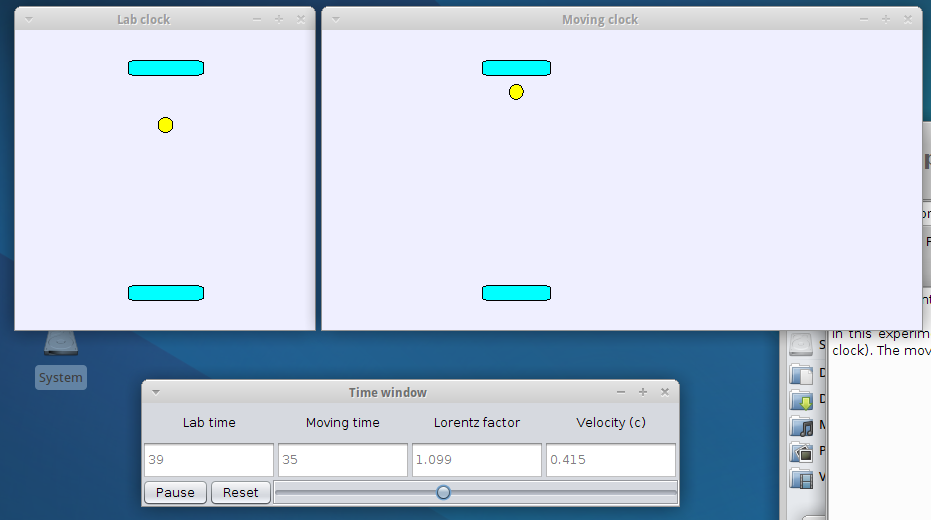
\includegraphics[width=.9\linewidth]{./mirrorUI.png}
\caption{UI of the photon clock simulation}
\end{figure}
\end{itemize} % ends low level

\end{document}
